In this chapter, we will discuss a number of activation functions.  We
say an activation function $\alpha$ 
satisfies the basic activated-approximation-property (AAP) if for any $g\in C^1[-1,1]$, we have
\begin{equation}
\label{AAP}
\min_{a_i,b_i,c,w_i\in\mathbb R^1}\max_{t\in[-1,1]}\bigg|g(t)-\sum_{i=1}^k(a_i\alpha(w_it+b_i)-c\bigg|
\le \frac{C}{k}\max_{t\in[-1,1]}|g'(t)|
\end{equation}
for some constant $C$ independent of $k$ and $g$. 

\section{Cardinal B-splines}
The {\it cardinal B-splines} are given by the following recurrent
relationship
\begin{equation}
  \label{cardinal}
M_d(x)=\frac{x}{d}M_{d-1}(x)  + \frac{d+1-x}{d}M_{d-1}(x-1)  
\end{equation}
\subsection{$d=0$}
\begin{equation}
  \label{cardinal}
M_0(x)=
\left\{
  \begin{array}{ll}
0 & x<0 \\
1 & 0\le x<1    \\
0 & x > 1    
  \end{array}
\right.
\end{equation}
The Heaviside function is defined by
\begin{equation}
  \label{a0}
\alpha_0(x)=
\left\{
  \begin{array}{ll}
0 & x<0; \\
1 & x \ge 1.
  \end{array}
\right.
\end{equation}
\begin{lemma}
  \begin{equation}
  \label{a0M0}
\alpha_0(x)=\sum_{j=0}^\infty M_0(x-j)    
  \end{equation}
  \begin{equation}
  \label{M0a0}
M_0(x)=\alpha_0(x)-\alpha_0(x-1).
  \end{equation}
\end{lemma}

\subsection{$d=1$}
\begin{equation}
  \label{M1M0}
M_1(x)=xM_0(x)+(2-x)M_0(x-1)  
\end{equation}
We note that
\begin{equation}
  \label{M1}
M_1(x)= 
\left\{
\begin{array}{cl}
0 & x<0; \\
x & 0\le x < 1\\
2-x & 1\le x \le 2\\
0 & x>2.
  \end{array}
\right.
\end{equation}
We define (see Fig. \ref{alpha1})
\begin{equation}
  \label{a1}
\alpha_1(x)= 
\left\{
\begin{array}{cl}
M_1(x) &  x < 1\\
1 & x\ge 1
  \end{array}
\right.
\end{equation}
\begin{figure}[!htb]
	\center{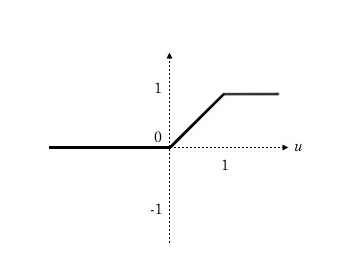
\includegraphics[width=10cm] {figures/alpha1.png}}        
	\caption{The activation $\alpha_1$}      
	\label{alpha1}
\end{figure}
 

\begin{lemma}
  \begin{equation}
    \label{a1a0}
\alpha_1(x)=x\alpha_0(x)+(1-x)\alpha_0(x-1).    
  \end{equation}
\end{lemma}

\begin{lemma}
  \begin{equation}
  \label{a1M1}
\alpha_1(x)=\sum_{j=0}^\infty M_1(x-j)    
  \end{equation}
\end{lemma}

\begin{lemma}
  \begin{equation}
    \label{M1a1}
M_1(x)=\alpha_1(x)-\alpha_1(x-1). 
  \end{equation}
\end{lemma}
Consider the following
$$
\alpha_1(x)-\alpha_1(2x-1). 
$$
We note that the so-called ReLU is defined as follows:
\begin{equation}
  \label{ReLU}
ReLU(x)= 
\left\{
\begin{array}{cl}
0 & x<0; \\
x & x\ge 0
  \end{array}
\right.
\end{equation}
and
\begin{equation}
\alpha_1(x)=ReLU(x)-ReLU(x-1).
\end{equation}

\begin{equation}
\alpha_1({1 \over h_1} x) - \alpha_1({1 \over h_2} (x - h_1) )
\end{equation}




\newpage
\subsection{$d=2$}
\begin{equation}
  \label{M2}
M_2(x)=\frac{x}{2}M_{1}(x)  + \frac{3-x}{2}M_{1}(x-1)   
\end{equation}
Note that
$$
M_2(0)=0, M_2(1)={1\over 2}, M_2({3\over2})={3\over 4},
M_2(2)={1\over2}, M_2(3)=0.
$$
Now we define
\begin{equation}
  \label{a2}
\alpha_2(x)= 
\left\{
\begin{array}{cl}
{4\over3}M_2(x) &  x < {3\over 2}\\
1 & x\ge {3\over2}
  \end{array}
\right.
\end{equation} 
Note that
$$
\alpha_2(0)=0, \alpha_2(1)={1\over 3}, \alpha_2({3\over2})=\alpha_2(2)=\alpha_2(3)=1.
$$
\begin{lemma}
 \begin{equation}
    \label{M2a2}
M_2(x)={3\over 2}(\alpha_2(x)-\alpha_2(x-1)).
  \end{equation}  
\end{lemma}
\begin{proof}
 We need to check some details ...
\end{proof}

\subsection{$d=3$}
The presentation below follows the file lect-spline.pdf found in the following web page
\begin{verbatim}
https://www.geos.ed.ac.uk/~yliu23/docs/lect_spline.pdf
\end{verbatim}
Take $x_0=0$ and $h=1$, we get
$$
B_0(x)=
\left\{
  \begin{array}{ll}
0 & x\le -2\\
\\
{1\over 6}(2+x)^3 & -2\le x\le -1\\ 
\\
{2\over 3}-{1\over2}x^2(2+x) & -1\le x\le 0\\  
\\
{2\over 3}-{1\over2}x^2(2-x) & 0\le x\le 1\\  
\\
{1\over 6}(2-x)^3 & 1\le x\le 2\\ 
\\
 0 & x\ge 2.    
  \end{array}
\right.
$$
Let 
$$
B_k(x)=B_0(x-k)
$$
A cubic spline function in $[0,N]$ can be written as
$$
S(x)=\sum_{k=-1}^{N+1}a_kB_0(x-k).
$$
The following identity holds:
\begin{equation}
  \label{eq:1}
\sum_{k=-1}^{N+1}B_0(x-k) =1, \quad\forall x\in [0,N]
\end{equation}
We propose the following activation function
$$
\sigma(x)=
\left\{
  \begin{array}{ll}
B_1(x) & x\le 1 \\
1 & x\ge 1    
  \end{array}
\right.
$$


\section{Approximation properties}
We consider an interval $I =(0,1)$ and a partition
\begin{equation}
  \label{1d-partition}
-1=t_0  < t_1<\ldots<t_k=1.
\end{equation}
As a special case of uniform partition, we take
\begin{equation}
\label{tk}
t_i=t_0+ih, I_i=(t_{i-1}, t_i)\quad i=1:k, h={2\over k}.  
\end{equation}
Consider the basis function 
$$
M_{0,i}(t)=M_0(\frac{t-t_{i-1}}{h}).
$$
Given 
$$
v: (-1,1)\mapsto \mathbb R^1
$$
The interpolation is defined as
\begin{equation}
  \label{interp0}
(\Pi_0v)(t) =\sum_{i=1}^kv_iM_{0,i}(t)
=v_1+\sum_{i=2}^k(v_i-v_1)M_{0,i}(t)
\end{equation}
with 
$$ 
v_i={1\over h}\int_{I_i}v(t).
$$
By \eqref{M0a0}, we have
\begin{eqnarray}
(\Pi_0v)(t)
&=&v_1+\sum_{i=2}^k(v_i-v_1)(\alpha_{0}(\frac{t-t_{i-1}}{h})-\alpha_{1}(\frac{t-t_{i}}{h}))\\
&=&v_1+\sum_{i=2}^k(v_i-v_1)(\alpha_{0}(\frac{t-t_{i-1}}{h})-\alpha_{0}(\frac{t-t_{i}}{h}))\\
&=&v_1+\sum_{i=1}^{k-1}(v_{i+1}-v_1)\alpha_{0}(\frac{t-t_{i}}{h})-
\sum_{i=2}^k(v_i-v_1)\alpha_{0}(\frac{t-t_{i}}{h})\\
&=&v_1+\sum_{i=1}^{k}(v_{i+1}-v_i)\alpha_{0}(\frac{t-t_{i}}{h}).
\end{eqnarray}
with 
$$
v_{k+1}=v_{1}.
$$
\begin{theorem}
  \label{M0-error}
  \begin{equation}
  \label{Pi0-error}
\|v-\Pi_0v\|_{0,\infty}\le \frac{c_0}{k}\|v'\|_{0,\infty}
\end{equation}
\end{theorem}
\begin{proof}
Easy.   
\end{proof}
In general, we consider the following space of Splines:
\begin{theorem}  \label{Md-error}

\subsection{General $d$}
Let $S^{d,k}$ be the spline space generated by the B-spline $M_d$ from
the partition \eqref{1d-partition}, we have
  \begin{equation}
  \label{Pid-error}
\|v-\Pi_{d,k}v\|_{0,\infty}\le \frac{c_d}{k^r}\|v^{(r)}\|_{0,\infty},
\quad 1\le r\le d+1.
\end{equation}
\end{theorem}
\begin{proof}
	You can find this proof in \cite{de1978practical} in theorem $XII.3$ in page 176.
It needs to be checked.  Li Lin might know where a proof can be found
in the literature. 
\end{proof}

\subsection{Sigmoidal function}
The so-called sigmoidal function is defined as follows:
\begin{equation}
  \label{sigmoidal}
\sigma(t) = \frac{1}{1 + e^{-t}}.  
\end{equation}
This popular activation provides a smooth approximation of the Heaviside function $\alpha_0$ as follows:
\begin{equation}
  \label{sig}
\lim_{a\to \infty}\sigma(at) = \alpha_0(t), \quad t\neq 0.
\end{equation}
For $t>0$
$$
\alpha_0(t)- \sigma(at)
=1-\frac{1}{1+e^{-at}}\le e^{-at}.
$$
For $t<0$
$$
\sigma(at)-\alpha_0(t)
=\frac{1}{1+e^{-at}}\le e^{-a|t|}.
$$
We have in general 
$$
|\sigma(at)-\alpha_0(t)|
\le e^{-a|t|}.
$$
We consider the following interpolation 
\begin{equation}
  \label{interp0-1}
v(t)=v_1+\sum_{i=1}  (v_i-v_1)
\end{equation}



%\newpage
\section{Special activation functions}

        \begin{itemize}
	\item An general activation function(must be nonlinear) is 
$$\sigma: \mathbb{R} \to  \mathbb{R}.$$

\item The Heaviside function is 
$$
H(x ) = \begin{cases}
0 \quad &\text{if} ~ x \le 0, \\
1 \quad &\text{if} ~ x > 0.
\end{cases}
$$
The biggest problem for this activation function is that this function is not continuous which will cause 
huge difficult in training phase.

\item The sigmoid function:
$$s(x) = \frac{1}{1 + e^{-x}}
\rightarrow 
\begin{cases}
0,~~x\rightarrow -\infty,\\
1,~~x\rightarrow +\infty.
\end{cases}
.
$$
This function can be seen as the smooth approximation of Heaviside function.
This activation function was very popular in shallow neural network in about 1990s. Now, this
activation function is also often used in RNN or some NLP tasks.


\item Currently, the most used activation function in DNN  and CNN is ``Rectified Linear Unit'' (ReLU):
$$
{\rm ReLU}(x) = \max(0, x).
$$
There are many interesting properties of ${\rm ReLU}$ function:
\begin{enumerate}
	\item ${\rm ReLU}$ is a piecewise linear function. Thus, DNN with this activation 
	function is always a piecewise linear function.
	
	\item The connection of ${\rm ReLU}$ and Heaviside.
	\begin{equation}
	\frac{d}{dx} {\rm ReLU}(x) = H(x).
	\end{equation}
	
	\item Recently, there are huge research works about the approximation properties of DNN
	with ${\rm ReLU}$ activation function see ~\cite{he2018relu,wang2018exponential,yarotsky2017error}.
\end{enumerate}
	
	\item The new activation function from ReLU is:
	$$
	\tau(x) = r(x) - r(x-1) = \begin{cases}
	0 \quad &\text{if} ~ x \le 0, \\
	x \quad &\text{if} ~  0 < x \le 1, \\
	1  \quad &\text{if} ~ x > 1.
	\end{cases}
	$$
        Here we need to note that, because $-r(x) \neq r(ax + b)$, so
        if we use $\tau$ as $f_{out}$, the layers will be $J+1$ for
        ReLU as activation function and $f_{out} = id$.
	\end{itemize}

Here is a simple diagram for a general DNN structure:
\begin{figure}[!h]
	\center{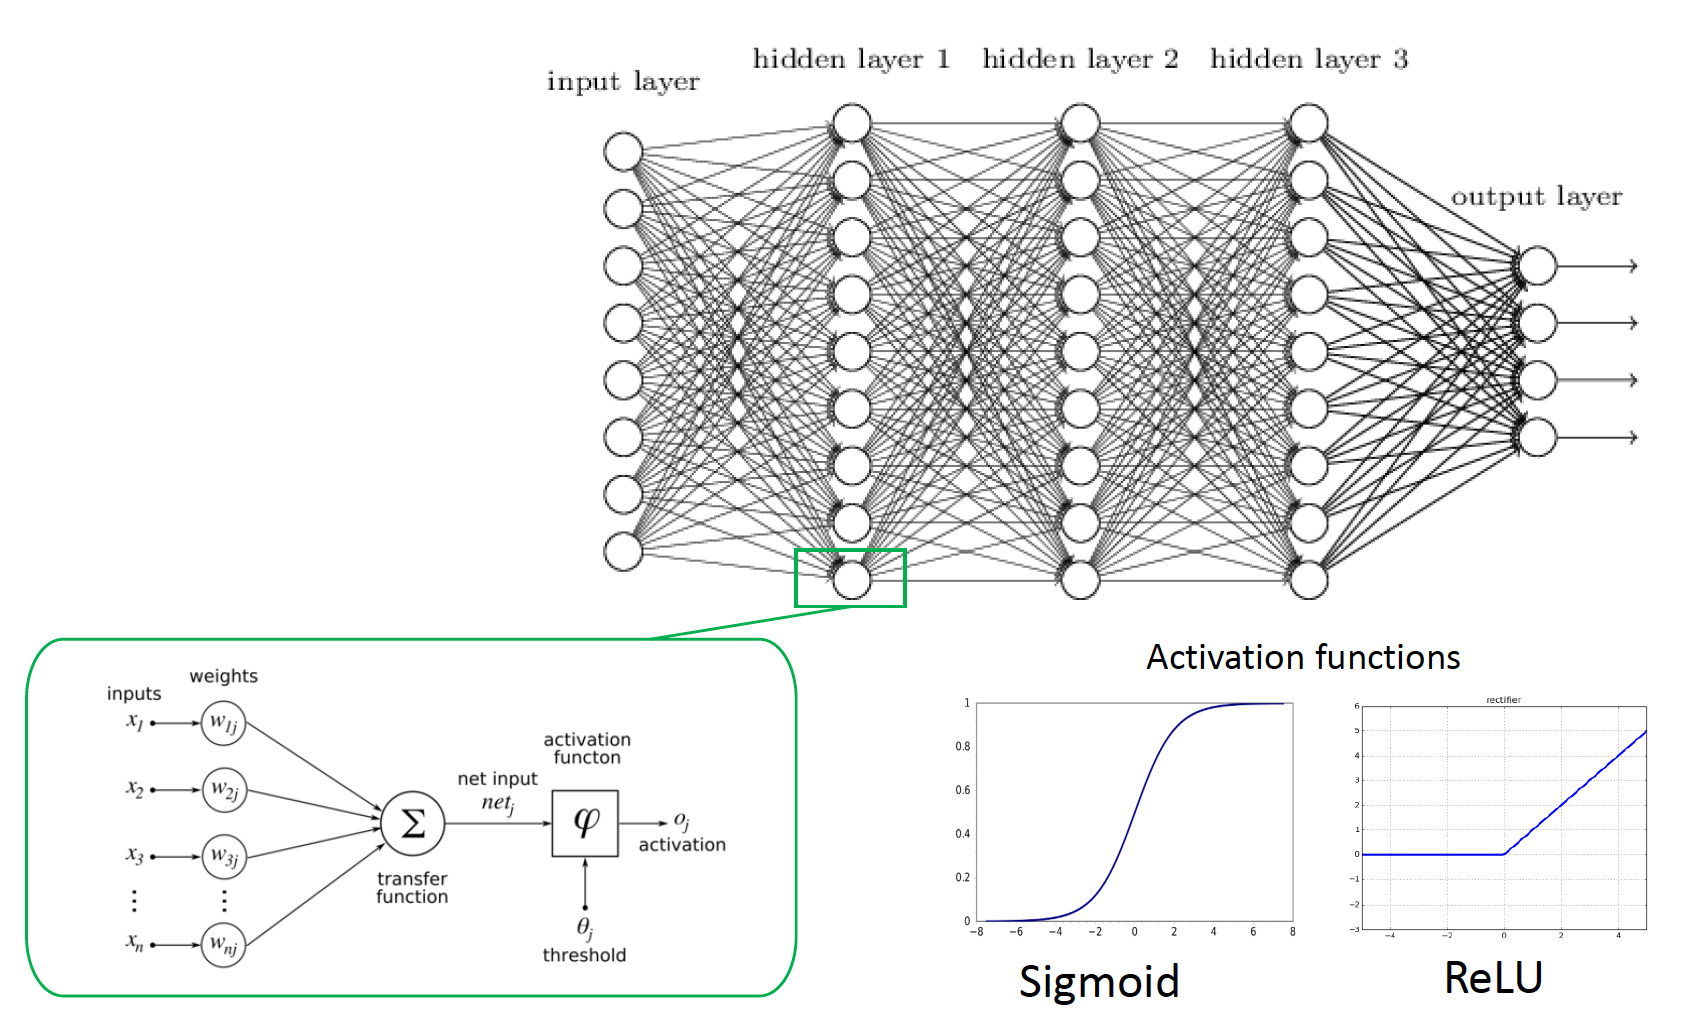
\includegraphics[width=12cm,height=6cm] {ANN.png}}
	\caption{A General Structure of DNN}
\end{figure}

